\section{Theorie}
\label{sec:Theorie}
Die Beugung von Licht lässt sich anhand des Huygensschen Prinzips modellieren. Hierbei
ist jeder Punkt der sich auszubreitenden Welle gleichzeitig der Ausgangspunkt einer neuen
Elementarwelle. Im Allgemeinen gibt es zwei Beugungsarten, die Fresnelsche und die Frauenhofersche Lichtbegung. 
Die Fresnelsche Lichtbeugung beschreibt eine Anordnung, bei der Lichtquelle und Beobachtungspunkt jeweils im Endlichen zu finden sind. 
Dies hat zur Konsequenz, das die Strahlen, die im Beobachtungspunkt $P$ interferieren jeweils unter verschiedenen Winkeln gebeugt werden (siehe Abbildung \ref{fig:Beugung}).
\begin{figure}[H]
    \centering
    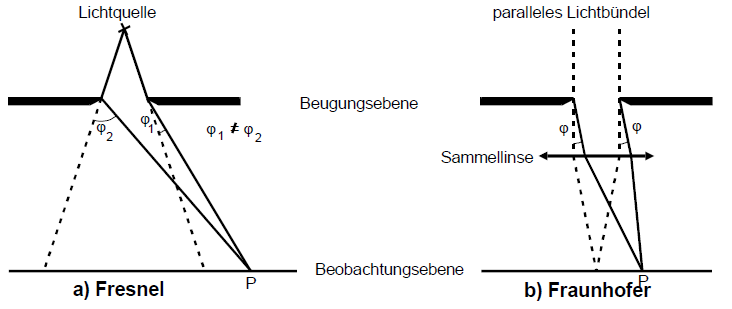
\includegraphics[width=0.8\textwidth]{Beugung.png}
    \caption{Beugungsarten \cite{1}.}
    \label{fig:Beugung}
\end{figure}
\noindent
Die Frauenhofersche Lichtbeugung hingegen geht von einer Lichtquelle mit unendlichen Abstand von der Beugungsebene aus, 
so das hier ein paralleles Lichtbündel mit einer ebenen Wellenfront vorhanden ist.
 Es falle nun eine ebene Welle mit der Feldstärke
\begin{equation} 
A(z,t)= A_0 \text{exp}\{i(wt-2\pi z/\lambda)\}
\end{equation}
pro Längeneinheit der Wellenfront aus der Z-Richtung ein.
Experimentell wird dies durch die Verwendung eines Lasers realisiert.
 Dies hat zur Folge, dass alle Strahlen die im Beobachtungspunkt $P$ ankommen und dort interferieren. 
 Diese werden unter dem selben Winkel gebeugt wurden und so werden diese drastisch vereinfacht. 
 Im Folgenden soll also nur noch die Frauenhofersche Lichtbeugung zur Lösung des Problemes herangezogen werden. 
 Hierbei sollte der Spalt zudem noch eine gro"se Länge gegen seine Breite aufweisen um nur eine Begrenzung 
 in eine Dimension zuzulassen und so die Beugungserscheinungen auf eine Dimension zu beschränken.\\
Um die Beugungserscheinungen zu erklären, wird eine Kombination aus dem Huygenschen Prinzip verwendet. 
Dies besagt, dass jeder Punkt einer Wellenfront Ursprung einer neuen Elementarwelle ist und dem Interferenzprinzip nach Fresnel, 
nach dem Wellen miteinander interferieren und eine neue Wellenfront bilden, welche der Einhüllenden der Elemetarwellen entspricht. 
\subsection{Beugung am Einzelspalt}
Zunächst werden zwei Strahlenbündel heraus gegriffen, die von zwei verschiedenen Punkten mit dem Abstand $x$ am Spalt ausgehen.
\begin{figure}[H]
    \centering
    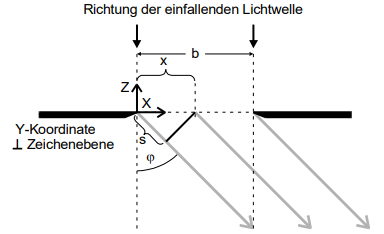
\includegraphics[width=0.5\textwidth]{einzel.png}
    \caption{Phasenbeziehung zwischen zwei Teilstrahlen bei der Frauenhoferschen Beugung am Spalt \cite{1}.}
    \label{fig:einzel}
\end{figure}
\noindent
 Durch ihren Wegunterschied $s$ kommt es zu einer Phasendifferenz von $\delta$:
\begin{equation}
\delta = \frac{2\pi s}{\lambda} = \frac{2 \pi x \sin\varphi}{\lambda}
\end{equation}
mit der Wellenlänge des Lichtes $\lambda$. Durch Integration über die Breite des Spaltes $b$ 
\begin{equation}
B(z,t,\varphi) = A_0 \int\limits_0^b \exp\left\{i\left(\omega t - \frac{2 \pi z}{\lambda} + \delta\right)\right\}dx
\end{equation}
($A_0$ ist die Amplitude der einfallenden Welle, $z$ die Wellenausbreitungsrichtung, $\omega$ die Frequenz und $t$ als Zeit) 
und Vernachlässigung unbedeutender Phasenfunktionen folgt schlie"slich 
\begin{align}
B(\varphi) = A_0b\frac{\sin\eta}{\eta}
\end{align}
mit der Abkürzung
\begin{align}
\eta := \frac{\pi b \sin\varphi}{\lambda}.
\end{align}
Die sich daraus ergebende Amplitudenfunktion entspricht der in Abbildung
\ref{fig:Amplitude} gezeigten Form wobei die Nullstellen bei
\begin{align}
    \text{sin} \phi_n &= \pm\, n \frac{\lambda}{b}
\end{align}
liegen.
\begin{figure}[H]
    \centering
    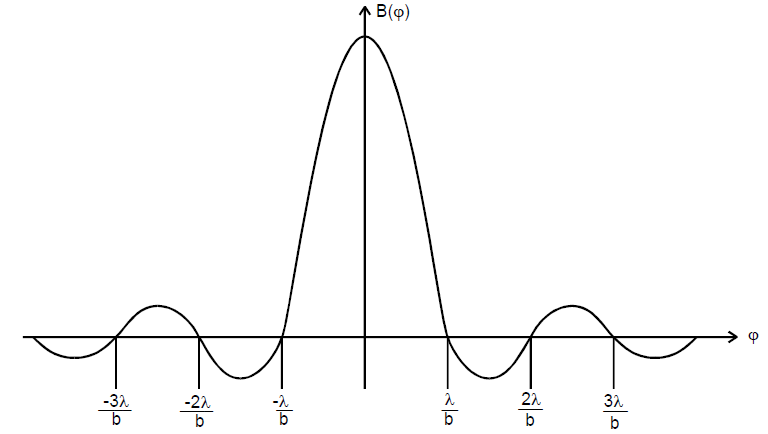
\includegraphics[width=0.8\textwidth]{Amplitude.png}
    \caption{Amplitudenfunktion am Parallelspalt \cite{1}.}
    \label{fig:Amplitude}
\end{figure}
\noindent
Aufgrund der hohen Lichtfrequenz von $\omega$ = $10^{14}$ bis $10^{15}$ Hz sind die Amplituden der Lichtwelle nicht direkt messbar.
 Die zeitlich gemittelte Intensität hingegen ist experimentell zugänglich, sie proportional zum Quadrat der Amplitudenfunktion. 
 \begin{equation}
I(\varphi) \propto B(\varphi)^2 = {A_0}^2 b^2 \left(
\frac{\lambda}{\pi b \sin (\varphi)} \right)^2 \sin^2 \left(
\frac{\pi b \sin (\varphi)}{\lambda} \right).
\end{equation}
\subsection{Beugung am Doppelspalt}
Die Beugung am Doppelspalt lässt sich in Analogie als Überlagerung zweier Einfach-Spalte der Breite $b$ im Abstand $s$ beschreiben. 
Der Aufbau ist schematisch in Abbildung \ref{fig:Doppelspalt} gezeigt.
\begin{figure}[H]
    \centering
    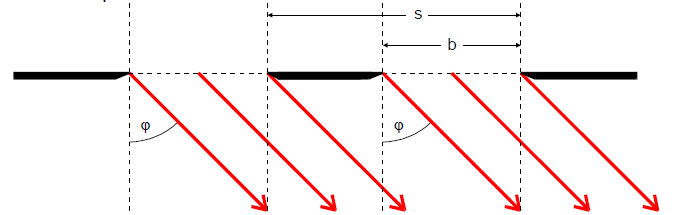
\includegraphics[width=0.8\textwidth]{Doppelspalt.png}
    \caption{Beugung am Doppelspalt \cite{1}.}
    \label{fig:Doppelspalt}
\end{figure}
\noindent
\begin{equation}
I(\varphi) \propto B(\varphi)^2 = 4 {A_0}^2 b^2 \cos^2 \left(
\frac{\pi s \sin (\varphi)}{\lambda} \right)  \left(
\frac{\lambda}{\pi b \sin (\varphi)} \right)^2 \sin^2 \left(
\frac{\pi b \sin (\varphi)}{\lambda} \right)
\end{equation}
Da sich die Intensitätsverteilung des Doppelspaltes aus der Intensitätsverteilung des Einfachspaltes und einer $\text{cos}^2$-Verteilung zusammensetzt,
  wird zusätzlich ein Minimum an den Nullstellen der $\text{cos}^2$-Verteilung beobachtet . 
\subsection{Frauenhofersche Beugung und Fourier-Transformation}
Die Funktion B($\varphi$) lässt sich als Fourier-Transformierte der Amplitudenverteilung der einfallenden Welle in der Beugungsebene
 (Aperturfunktion) ausdrücken. Allgemein wird  eine Fouriertransformation mit einer Funktion $f(x)$ so ausgedrückt:
 \begin{equation}
g(\xi) := \int\limits_{-\infty}^{+\infty}f(x)e^{ix\xi}dx.
\end{equation}
Am Spalt lässt sich die Aperturfunktion $f(x)$ als $f(x)$ = $A_0$ darstellen und durch einsetzen und Anwendung der Eulerschen Formel ergibt sich
\begin{equation}
g(\xi) = \frac{2A_0}{\xi}\exp\left(\frac{i\xi b}{2}\right)\sin\left(\frac{\xi b}{2}\right).
\end{equation}
Nun wird
\begin{align}
\xi := \frac{2\pi\sin\varphi}{\lambda}
\end{align}
eingesetzt, so beschreibt das die Fourier-Transformation das Huygensche Prinzip mathematisch. 
Vor allem sei zu beachten, dass durch die Umkehrbarkeit der Fourier-Transformation aus der Amplitudenfunktion
 die Gestalt $f(x)$ des beugenden Objektes berechnet werden kann.